\chapter{The Dinner}

It was evident that one sentiment affected all the guests on entering
the dining-room. Each one asked what strange influence had brought them
to this house, and yet astonished, even uneasy though they were, they
still felt that they would not like to be absent. The recent events,
the solitary and eccentric position of the count, his enormous, nay,
almost incredible fortune, should have made men cautious, and have
altogether prevented ladies visiting a house where there was no one of
their own sex to receive them; and yet curiosity had been enough to
lead them to overleap the bounds of prudence and decorum.

And all present, even including Cavalcanti and his son, notwithstanding
the stiffness of the one and the carelessness of the other, were
thoughtful, on finding themselves assembled at the house of this
incomprehensible man. Madame Danglars had started when Villefort, on
the count’s invitation, offered his arm; and Villefort felt that his
glance was uneasy beneath his gold spectacles, when he felt the arm of
the baroness press upon his own. None of this had escaped the count,
and even by this mere contact of individuals the scene had already
acquired considerable interest for an observer.

M. de Villefort had on the right hand Madame Danglars, on his left
Morrel. The count was seated between Madame de Villefort and Danglars;
the other seats were filled by Debray, who was placed between the two
Cavalcanti, and by Château-Renaud, seated between Madame de Villefort
and Morrel.

The repast was magnificent; Monte Cristo had endeavored completely to
overturn the Parisian ideas, and to feed the curiosity as much as the
appetite of his guests. It was an Oriental feast that he offered to
them, but of such a kind as the Arabian fairies might be supposed to
prepare. Every delicious fruit that the four quarters of the globe
could provide was heaped in vases from China and jars from Japan. Rare
birds, retaining their most brilliant plumage, enormous fish, spread
upon massive silver dishes, together with every wine produced in the
Archipelago, Asia Minor, or the Cape, sparkling in bottles, whose
grotesque shape seemed to give an additional flavor to the draught,—all
these, like one of the displays with which Apicius of old gratified his
guests, passed in review before the eyes of the astonished Parisians,
who understood that it was possible to expend a thousand louis upon a
dinner for ten persons, but only on the condition of eating pearls,
like Cleopatra, or drinking refined gold, like Lorenzo de’ Medici.

Monte Cristo noticed the general astonishment, and began laughing and
joking about it.

“Gentlemen,” he said, “you will admit that, when arrived at a certain
degree of fortune, the superfluities of life are all that can be
desired; and the ladies will allow that, after having risen to a
certain eminence of position, the ideal alone can be more exalted. Now,
to follow out this reasoning, what is the marvellous?—that which we do
not understand. What is it that we really desire?—that which we cannot
obtain. Now, to see things which I cannot understand, to procure
impossibilities, these are the study of my life. I gratify my wishes by
two means—my will and my money. I take as much interest in the pursuit
of some whim as you do, M. Danglars, in promoting a new railway line;
you, M. de Villefort, in condemning a culprit to death; you, M. Debray,
in pacifying a kingdom; you, M. de Château-Renaud, in pleasing a woman;
and you, Morrel, in breaking a horse that no one can ride. For example,
you see these two fish; one brought from fifty leagues beyond St.
Petersburg, the other five leagues from Naples. Is it not amusing to
see them both on the same table?”

“What are the two fish?” asked Danglars.

“M. Château-Renaud, who has lived in Russia, will tell you the name of
one, and Major Cavalcanti, who is an Italian, will tell you the name of
the other.”

“This one is, I think, a sterlet,” said Château-Renaud.

“And that one, if I mistake not, a lamprey.”

“Just so. Now, M. Danglars, ask these gentlemen where they are caught.”

“Sterlets,” said Château-Renaud, “are only found in the Volga.”

“And,” said Cavalcanti, “I know that Lake Fusaro alone supplies
lampreys of that size.”

“Exactly; one comes from the Volga, and the other from Lake Fusaro.”

“Impossible!” cried all the guests simultaneously.

“Well, this is just what amuses me,” said Monte Cristo. “I am like
Nero—\textit{cupitor impossibilium}; and that is what is amusing you at this
moment. This fish, which seems so exquisite to you, is very likely no
better than perch or salmon; but it seemed impossible to procure it,
and here it is.”

“But how could you have these fish brought to France?”

“Oh, nothing more easy. Each fish was brought over in a cask—one filled
with river herbs and weeds, the other with rushes and lake plants; they
were placed in a wagon built on purpose, and thus the sterlet lived
twelve days, the lamprey eight, and both were alive when my cook seized
them, killing one with milk and the other with wine. You do not believe
me, M. Danglars!”

“I cannot help doubting,” answered Danglars with his stupid smile.

“Baptistin,” said the count, “have the other fish brought in—the
sterlet and the lamprey which came in the other casks, and which are
yet alive.”

Danglars opened his bewildered eyes; the company clapped their hands.
Four servants carried in two casks covered with aquatic plants, and in
each of which was breathing a fish similar to those on the table.

“But why have two of each sort?” asked Danglars.

“Merely because one might have died,” carelessly answered Monte Cristo.

“You are certainly an extraordinary man,” said Danglars; “and
philosophers may well say it is a fine thing to be rich.”

“And to have ideas,” added Madame Danglars.

“Oh, do not give me credit for this, madame; it was done by the Romans,
who much esteemed them, and Pliny relates that they sent slaves from
Ostia to Rome, who carried on their heads fish which he calls the
\textit{mulus}, and which, from the description, must probably be the
goldfish. It was also considered a luxury to have them alive, it being
an amusing sight to see them die, for, when dying, they change color
three or four times, and like the rainbow when it disappears, pass
through all the prismatic shades, after which they were sent to the
kitchen. Their agony formed part of their merit—if they were not seen
alive, they were despised when dead.”

“Yes,” said Debray, “but then Ostia is only a few leagues from Rome.”

“True,” said Monte Cristo; “but what would be the use of living
eighteen hundred years after Lucullus, if we can do no better than he
could?”

The two Cavalcanti opened their enormous eyes, but had the good sense
not to say anything.

“All this is very extraordinary,” said Château-Renaud; “still, what I
admire the most, I confess, is the marvellous promptitude with which
your orders are executed. Is it not true that you only bought this
house five or six days ago?”

“Certainly not longer.”

“Well, I am sure it is quite transformed since last week. If I remember
rightly, it had another entrance, and the courtyard was paved and
empty; while today we have a splendid lawn, bordered by trees which
appear to be a hundred years old.”

“Why not? I am fond of grass and shade,” said Monte Cristo.

“Yes,” said Madame de Villefort, “the door was towards the road before,
and on the day of my miraculous escape you brought me into the house
from the road, I remember.”

“Yes, madame,” said Monte Cristo; “but I preferred having an entrance
which would allow me to see the Bois de Boulogne over my gate.”

“In four days,” said Morrel; “it is extraordinary!”

“Indeed,” said Château-Renaud, “it seems quite miraculous to make a new
house out of an old one; for it was very old, and dull too. I recollect
coming for my mother to look at it when M. de Saint-Méran advertised it
for sale two or three years ago.”

“M. de Saint-Méran?” said Madame de Villefort; “then this house
belonged to M. de Saint-Méran before you bought it?”

“It appears so,” replied Monte Cristo.

“Is it possible that you do not know of whom you purchased it?”

“Quite so; my steward transacts all this business for me.”

“It is certainly ten years since the house had been occupied,” said
Château-Renaud, “and it was quite melancholy to look at it, with the
blinds closed, the doors locked, and the weeds in the court. Really, if
the house had not belonged to the father-in-law of the procureur, one
might have thought it some accursed place where a horrible crime had
been committed.”

Villefort, who had hitherto not tasted the three or four glasses of
rare wine which were placed before him, here took one, and drank it
off. Monte Cristo allowed a short time to elapse, and then said:

“It is singular, baron, but the same idea came across me the first time
I came here; it looked so gloomy I should never have bought it if my
steward had not taken the matter into his own hands. Perhaps the fellow
had been bribed by the notary.”

“It is probable,” stammered out Villefort, trying to smile; “but I can
assure you that I had nothing to do with any such proceeding. This
house is part of Valentine’s marriage-portion, and M. de Saint-Méran
wished to sell it; for if it had remained another year or two
uninhabited it would have fallen to ruin.”

It was Morrel’s turn to become pale.

“There was, above all, one room,” continued Monte Cristo, “very plain
in appearance, hung with red damask, which, I know not why, appeared to
me quite dramatic.”

“Why so?” said Danglars; “why dramatic?”

“Can we account for instinct?” said Monte Cristo. “Are there not some
places where we seem to breathe sadness?—why, we cannot tell. It is a
chain of recollections—an idea which carries you back to other times,
to other places—which, very likely, have no connection with the present
time and place. And there is something in this room which reminds me
forcibly of the chamber of the Marquise de Ganges\footnote[10]{Elisabeth
de Rossan, Marquise de Ganges, was one of the famous women of the court
of Louis XIV. where she was known as “La Belle Provençale.” She was the
widow of the Marquis de Castellane when she married de Ganges, and having
the misfortune to excite the enmity of her new brothers-in-law, was
forced by them to take poison; and they finished her off with pistol
and dagger.—Ed.} or Desdemona. Stay, since we have finished dinner, I will
show it to you, and then we will take coffee in the garden. After dinner,
the play.”

Monte Cristo looked inquiringly at his guests. Madame de Villefort
rose, Monte Cristo did the same, and the rest followed their example.
Villefort and Madame Danglars remained for a moment, as if rooted to
their seats; they questioned each other with vague and stupid glances.

“Did you hear?” said Madame Danglars.

“We must go,” replied Villefort, offering his arm.

The others, attracted by curiosity, were already scattered in different
parts of the house; for they thought the visit would not be limited to
the one room, and that, at the same time, they would obtain a view of
the rest of the building, of which Monte Cristo had created a palace.
Each one went out by the open doors. Monte Cristo waited for the two
who remained; then, when they had passed, he brought up the rear, and
on his face was a smile, which, if they could have understood it, would
have alarmed them much more than a visit to the room they were about to
enter. They began by walking through the apartments, many of which were
fitted up in the Eastern style, with cushions and divans instead of
beds, and pipes instead of furniture. The drawing-rooms were decorated
with the rarest pictures by the old masters, the boudoirs hung with
draperies from China, of fanciful colors, fantastic design, and
wonderful texture. At length they arrived at the famous room. There was
nothing particular about it, excepting that, although daylight had
disappeared, it was not lighted, and everything in it was
old-fashioned, while the rest of the rooms had been redecorated. These
two causes were enough to give it a gloomy aspect.

“Oh.” cried Madame de Villefort, “it is really frightful.”

Madame Danglars tried to utter a few words, but was not heard. Many
observations were made, the import of which was a unanimous opinion
that there was something sinister about the room.

\begin{figure}[ht]
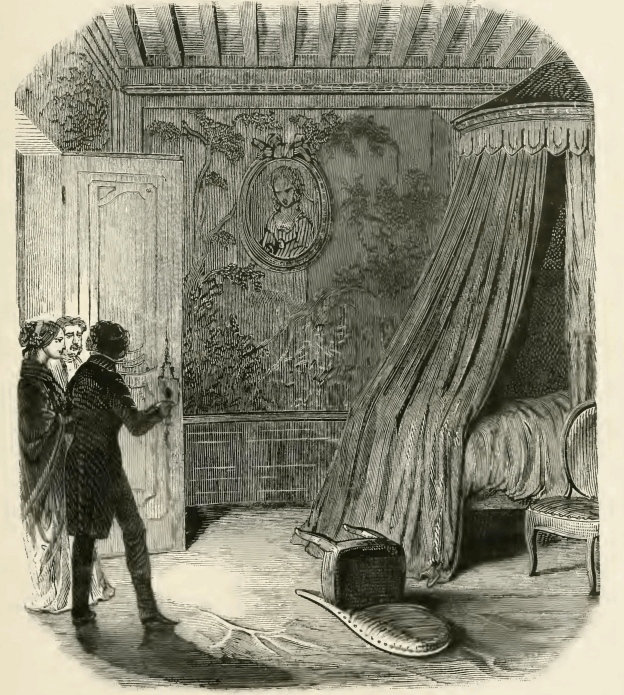
\includegraphics[width=\textwidth]{30221m.jpg}
\end{figure}

“Is it not so?” asked Monte Cristo. “Look at that large clumsy bed,
hung with such gloomy, blood-colored drapery! And those two crayon
portraits, that have faded from the dampness; do they not seem to say,
with their pale lips and staring eyes, ‘We have seen’?”

Villefort became livid; Madame Danglars fell into a long seat placed
near the chimney.

“Oh,” said Madame de Villefort, smiling, “are you courageous enough to
sit down upon the very seat perhaps upon which the crime was
committed?”

Madame Danglars rose suddenly.

“And then,” said Monte Cristo, “this is not all.”

“What is there more?” said Debray, who had not failed to notice the
agitation of Madame Danglars.

“Ah, what else is there?” said Danglars; “for, at present, I cannot say
that I have seen anything extraordinary. What do you say, M.
Cavalcanti?”

“Ah,” said he, “we have at Pisa, Ugolino’s tower; at Ferrara, Tasso’s
prison; at Rimini, the room of Francesca and Paolo.”

“Yes, but you have not this little staircase,” said Monte Cristo,
opening a door concealed by the drapery. “Look at it, and tell me what
you think of it.”

“What a wicked-looking, crooked staircase,” said Château-Renaud with a
smile.

“I do not know whether the wine of Chios produces melancholy, but
certainly everything appears to me black in this house,” said Debray.

Ever since Valentine’s dowry had been mentioned, Morrel had been silent
and sad.

“Can you imagine,” said Monte Cristo, “some Othello or Abbé de Ganges,
one stormy, dark night, descending these stairs step by step, carrying
a load, which he wishes to hide from the sight of man, if not from
God?”

Madame Danglars half fainted on the arm of Villefort, who was obliged
to support himself against the wall.

“Ah, madame,” cried Debray, “what is the matter with you? how pale you
look!”

“It is very evident what is the matter with her,” said Madame de
Villefort; “M. de Monte Cristo is relating horrible stories to us,
doubtless intending to frighten us to death.”

“Yes,” said Villefort, “really, count, you frighten the ladies.”

“What is the matter?” asked Debray, in a whisper, of Madame Danglars.

“Nothing,” she replied with a violent effort. “I want air, that is
all.”

“Will you come into the garden?” said Debray, advancing towards the
back staircase.

“No, no,” she answered, “I would rather remain here.”

“Are you really frightened, madame?” said Monte Cristo.

“Oh, no, sir,” said Madame Danglars; “but you suppose scenes in a
manner which gives them the appearance of reality.”

\begin{figure}[ht]
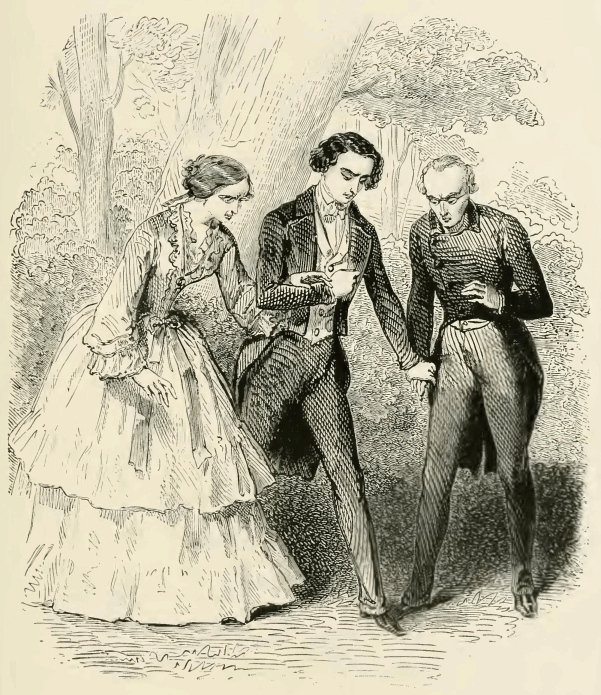
\includegraphics[width=\textwidth]{30223m.jpg}
\end{figure}

“Ah, yes,” said Monte Cristo smiling; “it is all a matter of
imagination. Why should we not imagine this the apartment of an honest
mother? And this bed with red hangings, a bed visited by the goddess
Lucina? And that mysterious staircase, the passage through which, not
to disturb their sleep, the doctor and nurse pass, or even the father
carrying the sleeping child?”

Here Madame Danglars, instead of being calmed by the soft picture,
uttered a groan and fainted.

“Madame Danglars is ill,” said Villefort; “it would be better to take
her to her carriage.”

“Oh, \textit{mon Dieu!}” said Monte Cristo, “and I have forgotten my
smelling-bottle!”

“I have mine,” said Madame de Villefort; and she passed over to Monte
Cristo a bottle full of the same kind of red liquid whose good
properties the count had tested on Edward.

“Ah,” said Monte Cristo, taking it from her hand.

“Yes,” she said, “at your advice I have made the trial.”

“And have you succeeded?”

“I think so.”

Madame Danglars was carried into the adjoining room; Monte Cristo
dropped a very small portion of the red liquid upon her lips; she
returned to consciousness.

“Ah,” she cried, “what a frightful dream!”

Villefort pressed her hand to let her know it was not a dream. They
looked for M. Danglars, but, as he was not especially interested in
poetical ideas, he had gone into the garden, and was talking with Major
Cavalcanti on the projected railway from Leghorn to Florence. Monte
Cristo seemed in despair. He took the arm of Madame Danglars, and
conducted her into the garden, where they found Danglars taking coffee
between the Cavalcanti.

“Really, madame,” he said, “did I alarm you much?”

“Oh, no, sir,” she answered; “but you know, things impress us
differently, according to the mood of our minds.” Villefort forced a
laugh.

“And then, you know,” he said, “an idea, a supposition, is sufficient.”

“Well,” said Monte Cristo, “you may believe me if you like, but it is
my opinion that a crime has been committed in this house.”

“Take care,” said Madame de Villefort, “the king’s attorney is here.”

“Ah,” replied Monte Cristo, “since that is the case, I will take
advantage of his presence to make my declaration.”

“Your declaration?” said Villefort.

“Yes, before witnesses.”

“Oh, this is very interesting,” said Debray; “if there really has been
a crime, we will investigate it.”

“There has been a crime,” said Monte Cristo. “Come this way, gentlemen;
come, M. Villefort, for a declaration to be available, should be made
before the competent authorities.”

He then took Villefort’s arm, and, at the same time, holding that of
Madame Danglars under his own, he dragged the procureur to the
plantain-tree, where the shade was thickest. All the other guests
followed.

“Stay,” said Monte Cristo, “here, in this very spot” (and he stamped
upon the ground), “I had the earth dug up and fresh mould put in, to
refresh these old trees; well, my man, digging, found a box, or rather,
the iron-work of a box, in the midst of which was the skeleton of a
newly born infant.”

\begin{figure}[ht]
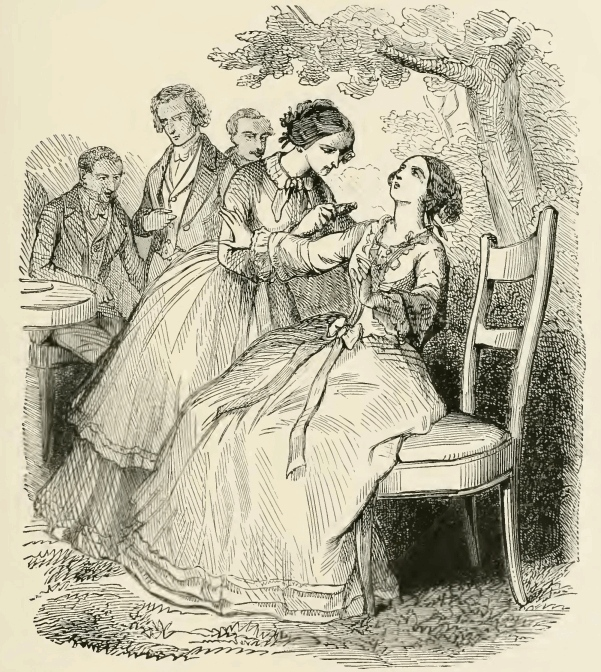
\includegraphics[width=\textwidth]{30225m.jpg}
\end{figure}

Monte Cristo felt the arm of Madame Danglars stiffen, while that of
Villefort trembled.

“A newly born infant,” repeated Debray; “this affair becomes serious!”

“Well,” said Château-Renaud, “I was not wrong just now then, when I
said that houses had souls and faces like men, and that their exteriors
carried the impress of their characters. This house was gloomy because
it was remorseful: it was remorseful because it concealed a crime.”

“Who said it was a crime?” asked Villefort, with a last effort.

“How? is it not a crime to bury a living child in a garden?” cried
Monte Cristo. “And pray what do you call such an action?”

“But who said it was buried alive?”

“Why bury it there if it were dead? This garden has never been a
cemetery.”

“What is done to infanticides in this country?” asked Major Cavalcanti
innocently.

“Oh, their heads are soon cut off,” said Danglars.

“Ah, indeed?” said Cavalcanti.

“I think so; am I not right, M. de Villefort?” asked Monte Cristo.

“Yes, count,” replied Villefort, in a voice now scarcely human.

Monte Cristo, seeing that the two persons for whom he had prepared this
scene could scarcely endure it, and not wishing to carry it too far,
said:

“Come, gentlemen,—some coffee, we seem to have forgotten it,” and he
conducted the guests back to the table on the lawn.

“Indeed, count,” said Madame Danglars, “I am ashamed to own it, but all
your frightful stories have so upset me, that I must beg you to let me
sit down;” and she fell into a chair.

Monte Cristo bowed, and went to Madame de Villefort.

“I think Madame Danglars again requires your bottle,” he said. But
before Madame de Villefort could reach her friend, the procureur had
found time to whisper to Madame Danglars, “I must speak to you.”

“When?”

“Tomorrow.”

“Where?”

“In my office, or in the court, if you like,—that is the surest place.”

“I will be there.”

At this moment Madame de Villefort approached.

“Thanks, my dear friend,” said Madame Danglars, trying to smile; “it is
over now, and I am much better.”
